\documentclass[10pt]{article}
\usepackage[margin=1in]{geometry}
\usepackage[T1]{fontenc}
\usepackage{lmodern}
\usepackage{microtype}
\usepackage{amsmath,amssymb}
\usepackage{booktabs}
\usepackage{graphicx}
\usepackage{xcolor}
\usepackage{url}
\usepackage[numbers,sort&compress]{natbib}
\usepackage[colorlinks=true,linkcolor=blue!50!black,citecolor=blue!50!black,urlcolor=blue!50!black]{hyperref}
\usepackage{caption}
\captionsetup{font=small}
\setlength{\emergencystretch}{2em}

\title{\textbf{Glance: Fast Typed Decisions about Images on a CPU}\\[4pt]
\large Technical report}
\author{Yuan Shen}
\date{September 2026}

\begin{document}
\maketitle

\begin{abstract}
Agents often need quick answers to small, typed questions about an image: yes or no, one of $K$ options, or a rating on a scale, each with a probability rather than generated text. We describe Glance, a family of encoders for such decisions, and release one of them, a 134M-parameter model trained only on data whose licences allow commercial use, under Apache-2.0. Questions are packed into isolated blocks over a cached image, and each candidate is isolated from the others and read out by mean-pooling its tokens; isolation and pooling each avoid one of two silent failure modes of slot-token readouts that we document. With ONNX Runtime on 4 CPU threads, the released model answers a question about a new photograph in 18.3\,ms on an Apple M4 Pro and 26.2\,ms on an AMD EPYC server, and a question about an image it has already seen in 3.0 and 4.1\,ms, in under 1\,GB of memory. On visible errors in AI-generated images the picture is mixed. It separates flawed generated images from real photographs as well as a research model trained on non-commercial error datasets (SalArt-VQA AUROC 0.911 for the released seed, 0.55--0.91 across three seeds of its recipe, against 0.904). Among generated images alone it ranks flawed above clean ones only moderately (AUROC 0.67 on ArtiBench, 0.70 on HAD, 0.83 on RichHF-18K). On SalArt's 119 pairs of a generated image and a version with a flaw inpainted, it scores the flawed one higher in 55\% of pairs (95\% interval 46--63\%), like the research models (48--51\%), and at its served threshold it flags 2.5\% of SalArt's real photographs but 78\% of the clean generated originals. It is well calibrated on everyday yes/no and two-way questions (smooth ECE 0.02--0.08), less so on four-way multiple choice (0.11--0.15), and on error benchmarks it ranges from well calibrated (0.05--0.09 on HAD any error and SalArt) to overconfident (0.21--0.35 on HAD hands, ArtiBench and RichHF). It is weak on open everyday questions (60\% on VQAv2 yes/no against 81\% for Qwen3-VL-2B). A slower research design reaches 69\%; none of five cheaper variants we tried recovers its advantage, which we attribute, without a direct test, to a vision-language backbone pretrained jointly at 512\,px. Audits of our data, training code, evaluation and this paper by separate reviewing agents found problems that the metrics did not show, including a label-parsing bug that made half of one source's negative labels false, a fairness failure invisible on our real-photo test set, a threshold tuned on the test set, and the question, which a paired test then answered, of whether our headline error benchmark measured flaws at all; we report them with the results. Code, weights and results: \url{https://github.com/benalive/glance}.
\end{abstract}

\section{Introduction}
Agents make many small decisions: whether a page has finished loading, whether a screenshot shows the expected result, whether a generated image has a malformed hand, how good an image is on a five-point scale. Each needs a probability over a few fixed answers, and they come up often enough that latency adds up. TypeSafe's Jev~\cite{jev2026,jevdocs} popularised this kind of model, a hosted service that answers \texttt{choice}, \texttt{noul} (yes/no) and \texttt{score} questions about a text state with a probability for every option. Open alternatives followed, the best known being Laya~\cite{laya2026}. Community measurements~\cite{sina2026} found that a local model gives more than ten times the decisions per second of the hosted API (86.5 against 3.2), largely because each API call, network and Jev's own inference together, takes about 300\,ms.

Image-aware open replicas exist (laya-vision~\cite{layavision2026}, visual-jev~\cite{visualjev2026} and others), but they are causal models of 0.45--8B parameters or carry non-commercial weights. Glance is an image-aware decision encoder designed around latency, with a fixed cost budget (about 30\,ms per new image and 5\,ms per additional question on a CPU, under 1\,GB, no GPU) and, for the released model, training data that can be redistributed in weights.

\paragraph{Contributions.}
\begin{itemize}\setlength\itemsep{1pt}
\item A typed-decision encoder design (\S\ref{sec:method}): isolated question blocks over a cacheable image context, candidate isolation with shared start positions (as in UniMC~\cite{unimc}), a mean-pooled pointer readout for all three answer types, and proper-scoring-rule training; and two failure modes of slot-token readouts that it avoids (\S\ref{sec:readout}).
\item Batch-1 latency measurements that separate per-layer cost from arithmetic on Apple silicon, and serving latency and memory of the released model on Apple silicon and x86 (\S\ref{sec:latency}).
\item A comparison of designs on vision-language decisions: the accurate design's lead is not recovered by earlier fusion, more image tokens, a pruned low-resolution copy of it, a partly trainable image encoder or more fusion layers (\S\ref{sec:designs}).
\item Visible-error detection in AI-generated images on published benchmarks, a distillation study, and a paired test showing that what our models detect on SalArt-VQA is mostly whether an image is generated, not whether it is flawed (\S\ref{sec:errors}).
\item An open-licence model and the process that produced it (\S\ref{sec:open}): per-image licence filtering, audits by separate reviewing agents and what they found, a partial mitigation of unreliable transfer to unseen question wordings, a fairness check and partial fix, calibration, and the released model next to every model we measured (Table~\ref{tab:final}).
\item A matched comparison with Laya on the community Snake benchmark (\S\ref{sec:snake}).
\end{itemize}

\section{Related work}
\paragraph{System~1 decision models.} Jev~\cite{jev2026,jevdocs} defines the interface we adopt: a state, a set of named questions, and typed answers with probabilities. Its architecture and training data are unpublished. Laya~\cite{laya2026} is an open, Jev-compatible text model built on ModernBERT-large (421M) or mmBERT-base (322M); LayaStudio~\cite{layastudio2026} fine-tunes it on a Mac with LoRA, and community ports run it with MLX~\cite{mlx2023,layamlx2026}. laya-vision~\cite{layavision2026} adds images through SmolVLM-256M~\cite{smolvlm} or ModernVBERT-250M and reports 32--41\,ms per image question in bf16 on an NVIDIA L4 GPU. visual-jev~\cite{visualjev2026} packs isolated question branches with a pointer head on a causal Qwen3-VL backbone; other community vision replicas are causal models of 0.45--8B parameters. Glance differs from laya-vision in isolating each question (laya-vision scores the questions of a request jointly), from visual-jev in being a bidirectional encoder and in isolating candidates from each other (visual-jev isolates questions but lets each option see the full list), and from both in caching the image across requests, targeting CPU latency, and releasing weights trained on licence-clean data. Causal models get a comparable cached-image path from prefix caching (RadixAttention in SGLang~\cite{sglang}), which visual-jev's shared-cache mode uses. Multiple-question multiple-answer VQA~\cite{mqma} already answers several questions in one encoder pass, without isolating them.
\paragraph{Encoders that score candidates jointly.} UniMC~\cite{unimc} puts all options in one sequence, masks attention between them and restarts their position ids; we use the same candidate isolation. GLiClass~\cite{gliclass} scores all labels in one pass but lets labels attend to each other; Set-Encoder~\cite{setencoder} and Set-LLM~\cite{setllm2025} make inputs order-invariant. M-FALCON~\cite{hstu2024} masks candidates from each other over a cached shared context in recommendation. Prompt Cache~\cite{promptcache} reuses the attention states of shared prompt segments across requests, DeFormer~\cite{deformer} caches question-independent lower layers, and EDJE~\cite{edje2025} runs a small joint encoder over cached vision tokens, close to our C5. Intra-prompt parallel decoding~\cite{ippd2026} answers several questions over one context in a single prompt, a decoder-side analogue of question packing.
\paragraph{Vision-language encoders.} ViLT~\cite{vilt} and VLMo~\cite{vlmo} feed patches and words into one transformer. ModernVBERT~\cite{modernvbert2025} combines a SigLIP~2~\cite{siglip2} vision encoder with an Ettin~\cite{ettin} (ModernBERT-style~\cite{modernbert}) text encoder, pretrained jointly; it is our quality reference. NeoMME~\cite{neomme} pretrains single-tower encoders from scratch on raw 32-pixel patches.
\paragraph{Visible errors in generated images.} HAD~\cite{hadm2024} annotates malformed body parts in images of people; RichHF-18K~\cite{richhf2024} has raters score artifacts and plausibility; EvalMuse-40K~\cite{evalmuse2024} marks structural problems in images from 20 generators; ImageReward~\cite{imagereward2023} collects fidelity ratings on Stable Diffusion images from DiffusionDB~\cite{diffusiondb2023}. SalArt-VQA~\cite{salart2026}, ArtiBench~\cite{artibench2026} and A-Bench~\cite{abench2024} evaluate vision-language models on detecting such errors and publish results for frontier models; SynthScars~\cite{legion2025} annotates flaws in generated images only. ArtifactLens~\cite{artifactlens2026} detects such artifacts from a few hundred labels on frozen vision-language models. Telling generated images from real ones is a separate and easier task: linear probes on frozen features already do it well~\cite{wang2020cnn,univfd2023}, which is what our SalArt analysis (\S\ref{sec:errors}) finds our error models doing.
\paragraph{Calibration, distillation and latency.} We train with the Brier score~\cite{brier1950} (the ranked probability score~\cite{epstein1969} for ordinal answers) plus cross-entropy, fit temperatures~\cite{guo2017} or Platt scaling~\cite{platt1999} on held-out data, and report smooth ECE~\cite{smece}. We distil with blended soft targets~\cite{hinton2015}. Framework overhead rather than arithmetic dominates batch-1 latency for small models~\cite{frameworktax}; depth-to-width ratio governs small-batch latency of small language models~\cite{nemotronflash2025}.

\section{Method}\label{sec:method}
\paragraph{Typed decisions.} A request carries an image and one or more questions. A question has a kind and candidates: \texttt{choice} with $2\le K\le 255$ named options, \texttt{noul} with \{yes, no\}, and \texttt{score} with one candidate per ordinal level, lowest first. The model returns a distribution over each question's candidates. A text state, as in Jev, is prefixed to each question; caching it like the image is designed but not built.

\paragraph{Packed sequence and masks.} A sequence is \texttt{[image][question 1]\dots[question $n$]}. A question block is \texttt{[CLS]}, the question tokens, then each candidate's tokens followed by a \texttt{[SEP]} slot. Positions restart in every block, and all candidates of a question start at the same position. A boolean mask enforces three rules: (1) image tokens attend only to image tokens, so their states do not depend on the questions and are computed once per image; (2) a question block attends to the image and to itself, never to another question, so a question gets the same answer alone or in a pack; (3) inside a block, question tokens see the whole block, but each candidate's tokens see only the question and themselves. Permuting a question's candidates then permutes its output probabilities exactly.

\paragraph{Readout and loss.} One pointer head serves all kinds. The question is summarised by its \texttt{[CLS]} state $h_q$ and candidate $k$ by the mean $\bar h_k$ of its own token states; the logit is $\ell_k = \langle W_c \bar h_k, W_q h_q\rangle/\sqrt{d}$, and a softmax over the question's candidates gives $p$. Against a possibly soft target $y$, the loss is $\sum_k (p_k - y_k)^2 + 0.3\,\mathrm{CE}(y,p)$, with the squared error replaced by the ranked probability score~\cite{epstein1969} over cumulative distributions for \texttt{score}. Both terms are strictly proper. After training we fit Platt scaling for yes/no (slope constrained non-negative) and a temperature for choice and score on held-out data.

\paragraph{Designs and naming.} Table~\ref{tab:cands} lists the designs. C1 is ModernVBERT (SigLIP~2 B/16 at 512\,px, pixel-shuffled to 64 tokens, into a 22-layer Ettin-150M); its vision side is frozen and cached. C3/C4 are single $12\times768$ towers with the shape of SigLIP~2 B/32, inherited or random. C5, the released design, keeps a frozen SigLIP~2 B/32 at 256\,px (64 cached image tokens) and trains an Ettin-32M text encoder, a projection, three cross-attention fusion layers and the head; only these run per question. Several C5 checkpoints appear below, named by their training data: the \emph{research C5} (trained with non-commercial data and distilled from C1, \S\ref{sec:errors}) and the \emph{released C5} (licence-clean data only, \S\ref{sec:open}).

\begin{table}[t]
\centering\footnotesize
\caption{Designs. Depth: sequential layers per request with a new image / a cached image. C7--C9 and the C5 variants are defined in \S\ref{sec:designs}.}
\label{tab:cands}
\setlength\tabcolsep{4pt}
\begin{tabular}{llrrl}
\toprule
ID & Design & Params & Depth new / cached & Initialisation \\
\midrule
C1 & ModernVBERT: SigLIP~2 B/16 @512\,px $\to$ Ettin-150M & 252M & 34 / 22 & inherited \\
C2 & C1, text stack pruned to 11 layers, 256\,px & 197M & 23 / 11 & inherited \\
C3 & single tower $12\times768$, per-modality FFN & 183M & 12 / 12 & SigLIP~2 B/32 \\
C4 & C3 shape & 183M & 12 / 12 & random \\
C5 & frozen SigLIP~2 B/32 @256, Ettin-32M, 3 fusion layers & 134M & 25 / 13 & inherited \\
C6 & single tower $6\times512$ & 59M & 6 / 6 & random \\
\bottomrule
\end{tabular}
\end{table}

\section{Latency}\label{sec:latency}
\paragraph{Where the time goes.} On an Apple M4 Pro at batch 1 in eager PyTorch (15 warm-up and 60 timed iterations, median, random weights), a grid of plain pre-norm encoders (depth 2--22, width 256--1024, 128 or 384 tokens) is fit with $R^2=0.999$ by a fixed cost per layer plus a cost per GFLOP:
\begin{align*}
\text{GPU (MPS, fp16):}&\quad t \approx 0.11 + 0.244\,L + 0.159\,G \ \text{ms},\\
\text{CPU (fp32, 4 threads):}&\quad t \approx -0.10 + 0.519\,L + 0.521\,G \ \text{ms},
\end{align*}
where $L$ is the number of sequential layers and $G$ the GFLOPs. Either term alone fits much worse ($R^2$ 0.96--0.97 for GFLOPs, 0.43--0.50 for depth). The per-layer cost equals about 1--1.5 GFLOPs of arithmetic, so it dominates models that do little arithmetic per layer (Figure~\ref{fig:depth}). C1 at 512\,px spends most of its time in its 16\,px-patch vision stem (243 GFLOPs for a new image); a 32\,px stem at 256\,px needs 11. Once the image is cached, the per-layer term dominates every Glance design.

\begin{figure}[t]
\centering
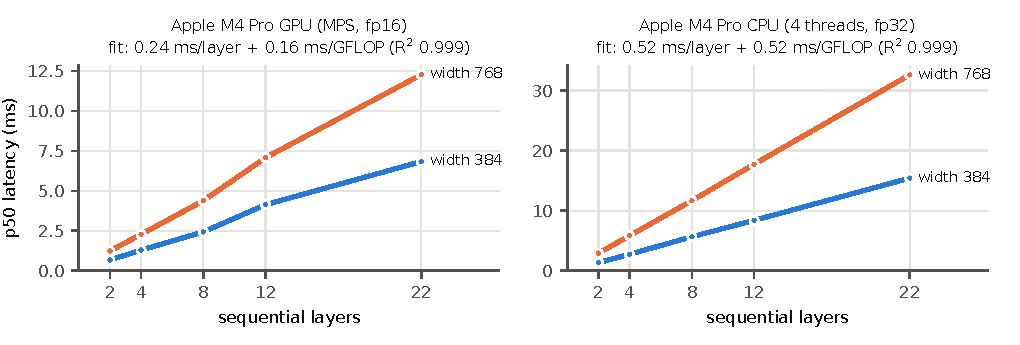
\includegraphics[width=0.85\linewidth]{figures/latency_depth.pdf}
\caption{Batch-1 p50 latency of plain encoders at 128 tokens against sequential layers, for two widths, on an Apple M4 Pro; titles give the per-device fit over the full grid.}
\label{fig:depth}
\end{figure}

\paragraph{Serving the released model.} Table~\ref{tab:serve} times the released model through the server's own code path (image decode and resize, image encoder, packing, model, calibration; HTTP excluded) on 30--40 COCO photographs, batch 1, 4 threads, on an otherwise idle machine; runs vary by 10--20\%. In eager PyTorch the M4 Pro is within the budget (23.0\,ms per new image, 5.1\,ms per cached-image request) and an x86 server (a cloud VM with an AMD EPYC 9V45, AVX-512) is not (57.3\,ms). On x86, int8 dynamic quantisation is fastest but changes 13\% of confident answers (10 of 78; 10\% on the M4 Pro); bf16 halves new-image time with small drift (largest change in $P(\text{yes})$ 0.049, no flipped answer); \texttt{torch.compile} gives no gain; and exporting both the image path and the question path to ONNX Runtime~\cite{onnxruntime} gives the largest exact speed-up (largest change in $P(\text{yes})$ 0.0001; on 300 held-out questions, largest logit change $5\times10^{-4}$ and no changed answer). Each further question in the same request adds 0.3--0.7\,ms on the M4 Pro and 1.2--1.4\,ms on the EPYC. With 32 threads, ONNX Runtime on the EPYC was 6.3--6.9$\times$ slower for new images (181\,ms) and 2.6--3.9$\times$ slower for cached-image requests, so the default stays at 4; PyTorch, in contrast, gets faster with 32 threads (32.4\,ms per new image) but stays slower than ONNX Runtime at 4. Peak memory of a serving process is 959\,MB with ONNX Runtime and 1.45\,GB with PyTorch. The budget verdicts for the designs in \S\ref{sec:designs} were made under eager PyTorch before the ONNX export existed.

\begin{table}[t]
\centering\footnotesize
\caption{Serving latency (median ms, batch 1). Top: the released model, served code path, 4 threads, 30--40 COCO photographs $\le$512\,px, otherwise idle machine. Bottom: reference points under their own protocols (SmolVLM and Qwen: model only, 64 image tokens), not directly comparable with the top rows or with each other.}
\label{tab:serve}
\setlength\tabcolsep{3pt}
\begin{tabular}{lllrr}
\toprule
Model & Machine & Runtime & New image & Cached image \\
\midrule
Glance C5 (released) & Apple M4 Pro CPU & ONNX Runtime & 18.3 & 3.0 \\
Glance C5 (released) & AMD EPYC 9V45 CPU & ONNX Runtime & 26.2 & 4.1 \\
Glance C5 (released) & Apple M4 Pro CPU & PyTorch fp32 & 23.0 & 5.1 \\
Glance C5 (released) & AMD EPYC 9V45 CPU & PyTorch fp32 & 57.3 & 7.3 \\
\midrule
Glance C1, research (served path, RichHF images) & Apple M4 Pro CPU & PyTorch fp32 & 166.5 & 24.1 \\
SmolVLM-256M (random weights) & M4 Pro CPU / GPU & PyTorch & 183.0 / 55.3 & 23.0 / 12.7 \\
Qwen3-VL-2B (random weights) & Apple M4 Pro GPU & PyTorch fp16 & 135.0 & 81.1 \\
Laya-snake 322M (one text decision, no image) & Apple M4 Pro CPU & PyTorch & 40.3 & -- \\
laya-vision (published) & NVIDIA L4 GPU & PyTorch bf16 & 32--41 & -- \\
\bottomrule
\end{tabular}
\end{table}

\section{Two failure modes of slot-token readouts}\label{sec:readout}
Our first implementation read each candidate from its closing \texttt{[SEP]} slot. It failed in two ways, neither raising an error. \textbf{Collapse:} when candidates share a start position and every token attends to every other, the slots of two equal-length candidates are identical at every layer, so every yes/no answer was exactly 0.5; overfitting one batch stalled at a loss of 0.70 instead of the 0.027 floor. Candidate isolation (rule 3) breaks the symmetry. A permutation-invariance test passed throughout, because collapsed outputs are trivially invariant. \textbf{Saddle:} with isolation, slots differ only through weak attention to their own words; a randomly initialised $4\times256$ tower had slot states with cosine similarity 0.999996, and since the head's gradient is $h_q\otimes g_0(h_0-h_1)$ for two candidates, gradients reaching the tower were about $10^{-7}$. Towers with a language-pretrained text path escape this; the single towers C3, C4 and C6 did not. Mean-pooling each candidate's tokens separates candidates from the embedding layer onwards and raised the initial gradient to 0.3.

\section{Which design, and why the accurate one is slow}\label{sec:designs}
\paragraph{Setup.} C1--C8 were trained on the same 119k decisions from public datasets (VQAv2~\cite{vqav2}, A-OKVQA~\cite{aokvqa}, COCO~\cite{coco} object presence, KonIQ~\cite{koniq}), with learning rates chosen on a 2\% development split for C1--C6 (C7 and C8 at C5's rate). C9 was trained on the distillation mix of \S\ref{sec:errors}, and C5u4 and C5f6 on the licence-clean mix of \S\ref{sec:open}, each compared against a C5 trained on the same data. Evaluation uses held-out benchmarks: POPE~\cite{pope}, A-OKVQA, MMStar~\cite{mmstar}, SugarCrepe~\cite{sugarcrepe}, KonIQ-10k, and 6{,}813 VQAv2 validation yes/no questions on 2{,}840 images outside every training mix (``everyday yes/no''), of which the report split scored here has 5{,}336 on 2{,}276 images once 5--5 annotator ties are excluded. In this section, yes/no accuracy uses a threshold fitted on each benchmark's own calibration split and scored on its report split, which is fair between runs but not comparable with published results. All runs are single seeds. These research models were trained on images with non-commercial licences and are not released.

\paragraph{Results.} At half an epoch, C1 led (development accuracy 0.791), C5 was the best fast design (0.697), C2 reached 0.69, and the single towers C3, C4 and C6 stayed near chance (0.47--0.53) even with the mean-pooled readout. After two epochs, C1 and C5 differ most on everyday questions: VQAv2 yes/no 0.701 vs.\ 0.554, A-OKVQA 0.606 vs.\ 0.433, SugarCrepe relation / attribute 0.717 / 0.756 vs.\ 0.637 / 0.577; C5 ranks image quality slightly better (KonIQ SRCC 0.815 vs.\ 0.801). C5 fits VQAv2 yes/no only to 0.615 on its own training questions, against 0.95 for object presence, which suggests the limitation lies in the model rather than in calibration.

\paragraph{Five cheaper variants.} None recovers C1's accuracy within the budget.
\begin{itemize}\setlength\itemsep{1pt}
\item \textbf{Earlier fusion at C5's size} (C7: image tokens fed into every Ettin-32M layer; 24.0\,ms per new image): below C5 on most benchmarks (POPE-adv 0.737 vs.\ 0.791, VQAv2 0.538 vs.\ 0.554).
\item \textbf{More image tokens} (C8: SigLIP~2 B/16 at 256\,px, 256 tokens): modestly better (VQAv2 0.576, POPE-adv 0.813) at 43.3\,ms per new image in eager PyTorch.
\item \textbf{C1 cut down} (C9: 192\,px, 6 of 22 text layers, initialised from C1; 35.0\,ms): below C5 on everything (POPE-adv 0.566). Resolution is the cause: unpruned C1 fed 192\,px images scores POPE AUROC 0.524 (0.901 at 512\,px), and a linear probe on its 192\,px features drops from 0.97 to 0.82 AUROC on RichHF artifacts. C1's vision side needs its 512\,px input, about 150\,ms on the CPU.
\item \textbf{Training the top of the image encoder} (C5u4: SigLIP's top 4 layers trainable; same inference cost): worse than the matched C5 on VQAv2 at the inherited learning rate ($-0.030$ [$-0.043$, $-0.017$]) and at a fifth of it ($-0.019$ [$-0.032$, $-0.007$]); at the higher rate it also fits its own training data worse.
\item \textbf{More fusion layers} (C5f6: six instead of three): POPE-adv $+0.015$ [$+0.002$, $+0.028$], VQAv2 $+0.006$ [$-0.004$, $+0.017$], SugarCrepe attribute $-0.042$ [$-0.090$, $+0.006$], at 6.0\,ms per cached-image request in eager PyTorch.
\end{itemize}
Brackets are paired, image-grouped bootstrap 95\% intervals (2{,}000 resamples, seed 0). A larger text encoder in C5 raised the cached-image request to 10.1\,ms (Ettin-68M) or 18.3\,ms (Ettin-150M), measured with untrained weights in eager PyTorch. C1 differs from C5 in several ways at once: a vision-language backbone pretrained jointly, 512\,px input with 16\,px patches, and a deeper, wider text stack. The variants rule out fusion depth, more tokens at 256\,px and a low-resolution copy of C1; we attribute the remaining gap to joint pretraining at 512\,px, but have not tested that directly.

\section{Visible errors in AI-generated images}\label{sec:errors}
\paragraph{Research models.} Zero-shot, the models we tried were weak at telling whether an AI image has visible errors (Qwen3-VL-2B AUROC 0.59--0.65 below), yet a linear probe on C5's frozen image features separates flawed from clean images (AUROC 0.79 on HAD hands, 0.96 on RichHF artifacts): the features carry the signal. Fine-tuning C5 on HAD~\cite{hadm2024} and RichHF-18K~\cite{richhf2024} (no stated licence; research use only), with about eight wordings per polarity, real photographs as negatives and replay of the general data, gives AUROC 0.778 (hands), 0.790 (any anatomy error) and 0.915 (RichHF artifacts) before distillation (the distilled research C5 in Table~\ref{tab:final}: 0.781 / 0.802 / 0.912), against 0.638 / 0.593 / 0.652 for Qwen3-VL-2B zero-shot. Without real negatives, 62\% of real photos were flagged.

\paragraph{Published benchmarks.} SalArt-VQA~\cite{salart2026} asks whether an image has a salient artifact; we score 437 flawed images and 318 real photographs after removing 38 derived from HAD (the published rows use 475 and 356; SalArt's paper mentions 30 HAD images, and we follow the released data). ArtiBench~\cite{artibench2026} has 1{,}000 generated images, half flawed; A-Bench~\cite{abench2024} asks descriptive multiple-choice questions. Glance receives the benchmark's short question and is read from its option probabilities with a calibration fixed before these benchmarks were run; the published rows used long instruction prompts and graded generated text, so they are reference points rather than a controlled comparison. The research C5 scores 83.0\% on SalArt Q1 (Gemini 3.1 Pro 78.3, Gemini 3.1 Flash Lite 87.6, Claude 4.6 Opus 70.0, GPT-5.4 45.5) and 0.584 on ArtiBench (GPT-4o 0.619, GPT-5 0.599; ArtiBench's own fine-tuned open models, the best published rows, 0.627 for Qwen2.5-VL-7B and 0.630 for InternVL3.5-8B). Neither Glance model can say where an error is (SalArt's region questions are near chance) or answer A-Bench's descriptive options (29.6\% for the research C5, 36.4\% for the release, on the 250 generative-distortion questions of its validation split; chance 34.9\%).

\paragraph{Distillation.} C1 fine-tuned on the same error data is slightly better at error detection (SalArt AUROC 0.928) but 7$\times$ slower. We labelled all 286k training questions with its probabilities and trained C5 on 50/50 blended targets~\cite{hinton2015}. Against a control trained on the same data with gold targets only, the teacher helps on SalArt (AUROC $+0.083$ [$+0.061$, $+0.104$]) and nowhere else measurably (ArtiBench $+0.012$ [$-0.005$, $+0.029$], VQAv2 yes/no AUROC $+0.005$ [$-0.002$, $+0.013$]).

\paragraph{Flawed, or generated?} SalArt's Q1 score compares 437 flawed generated images with 318 real photographs: its 119 unflawed generated images have no Q1 answer and are left out of the benchmark. Those 119 are the originals of 119 of the flawed images, into which SalArt inpainted a flaw (96 from Imagen~4, 23 from three other generators). The inpainting re-renders a region (a median of 12\% of pixels change), so each pair differs in the flaw and in that re-rendered region. We asked every Glance model Q1 about the originals as well (Table~\ref{tab:pairs}, served path). Within pairs, the release gives the flawed image the higher P(yes) in 65 of 119 pairs (0.55, 95\% interval 0.46--0.63), the research C5 and C1 in 0.51 and 0.48 (\path{results/salart_breakdown.json}); 119 pairs cannot rule out a modest effect, but none is evident. The research models flag 97--98\% of the clean originals and the release 78\%. Pooled over all clean originals the AUROC falls below 0.5 (0.27--0.46), but that reflects the generator mix: 96 of the originals are Imagen~4 images, which every model scores high, and within Imagen~4 alone flawed against clean is 0.46--0.52. The release's recall on SalArt's flawed images also depends on the generator: 75\% on Imagen~4 against 20--38\% on the FLUX, Z-Image and Qwen images. The high SalArt AUROC therefore mostly measures how well a model separates generated images from real photographs. Frozen image features do differ within pairs in a consistent direction (a linear direction fit on other pairs orders 90\% of held-out pairs at 256\,px and 96\% at 512\,px), but a probe on single images reaches only 0.56--0.57, and the direction may reflect the re-rendering rather than the flaw (\path{results/pair_probe.json}). Resolution alone does not explain the result: C1 at 512\,px also scores chance, and scoring the release on zoomed $2\times2$ or $3\times3$ tiles (maximum over tiles) leaves it at 0.51. We also retrained the release's second stage with 3{,}959 procedural local anomalies in clean generated images (a duplicated, twisted, torn or foreign patch, in the spirit of CutPaste~\cite{cutpaste}), each paired with a control that went through the same blend unchanged (one seed; 7\% more steps than the release's second stage): the model learned them (held-out pairs 0.54 $\to$ 0.80, controls still scored like untouched originals), but SalArt's pairs stayed at 0.51, the error benchmarks got worse by more than the spread across the released recipe's seeds (HAD 0.70 $\to$ 0.67, RichHF 0.83 $\to$ 0.76, ArtiBench 0.67 $\to$ 0.63), and everyday benchmarks slightly (VQAv2 0.600 $\to$ 0.594), so the release keeps the original recipe. Benchmarks made only of generated images are the better guide to flaw detection: ArtiBench 0.63--0.67, HAD 0.70--0.80 and RichHF 0.83--0.94 (Table~\ref{tab:final}; HAD and RichHF are in-distribution for the research models).

\begin{table}[t]
\centering\footnotesize
\caption{SalArt-VQA Q1 with its 119 clean generated originals added, through the served CPU path with each model's calibration (release seeds 1 and 2: no calibration, AUROC only). Served values differ slightly from the offline ones in Table~\ref{tab:final} (SalArt AUROC 0.913 vs 0.911 for the release; 0.570 vs 0.551 for seed 1). Flawed vs real is the benchmark's usual comparison; flawed vs original pools the 119 inpainted images and their originals; flawed vs clean AI mixes generators (see text).}
\label{tab:pairs}
\setlength\tabcolsep{4pt}
\begin{tabular}{lcccccc}
\toprule
 & \multicolumn{3}{c}{AUROC} & \multicolumn{3}{c}{Flagged at served threshold} \\
\cmidrule(lr){2-4}\cmidrule(lr){5-7}
Model & flawed vs real & flawed vs original & flawed vs clean AI & flawed & real & clean AI \\
\midrule
Glance C5 released (seed 0) & 0.913 & 0.508 & 0.284 & 44.9\% & 2.5\% & 78.2\% \\
Glance C5, recipe seed 1 / seed 2 & 0.570 / 0.887 & 0.509 / 0.506 & 0.456 / 0.271 & -- & -- & -- \\
Glance C5 research & 0.905 & 0.501 & 0.335 & 79.2\% & 10.7\% & 98.3\% \\
Glance C1 research & 0.929 & 0.495 & 0.332 & 82.4\% & 10.1\% & 97.5\% \\
\bottomrule
\end{tabular}
\end{table}

\section{An open-licence model}\label{sec:open}
The models above cannot be released: 69\% of COCO training photos carry NonCommercial terms, KonIQ-10k, HAD and RichHF-18K state no usable licence, and every checkpoint and teacher inherits this. We retrained from the public base models (SigLIP~2, Apache-2.0; Ettin, MIT).

\paragraph{Data.} Photos: the 13{,}543 COCO training photos licensed CC BY 2.0, ``no known copyright restrictions'' or US Government work (per-image licence from the official annotations; NonCommercial, NoDerivs and ShareAlike excluded), and 28{,}920 Open Images~\cite{openimages2020} photos (CC BY 2.0). Questions: VQAv2 and GQA~\cite{gqa2019} (CC BY 4.0; GQA's Visual Genome~\cite{visualgenome2017} images mapped to the same COCO photos), A-OKVQA (Apache-2.0), object presence from COCO labels and Open Images' human-verified positive and negative labels, and synthetic quality scores from graded distortions (KonIQ's replacement). AI images with human flaw labels: EvalMuse-40K~\cite{evalmuse2024} from the 13 open-weight generators whose output licences permit this use (closed generators and those restricting use of their outputs excluded after reading each licence) and ImageRewardDB~\cite{imagereward2023} (Apache-2.0; its Stable Diffusion images come from DiffusionDB, CC0). Every training image has an attribution record. Training photos were matched against every evaluation image by COCO id, Flickr id and a perceptual hash, and matches removed; face crops added later were matched against FairFace by perceptual hash only. In experiments (below), Qwen3-VL-2B~\cite{qwen3vl} (Apache-2.0) served as a teacher for everyday questions; the released model uses no teacher.

\paragraph{What the audits caught.} Separate reviewing agents (language-model sessions given the repository and an audit brief, run apart from the sessions that produced the results) reviewed the data, the training code, the evaluation and this paper, and found problems that the metrics did not show. Some earlier internal claims were corrected as a result; the results below are after all corrections.
\begin{itemize}\setlength\itemsep{1pt}
\item Open Images' label files write ``present'' as either \texttt{1} or \texttt{1.0}; reading only the former made 48.6\% of the ``no'' answers objects that were present (28{,}199 wrong decisions, 13\% of the mix). The first baseline run was discarded.
\item Text-only shortcuts: GQA ``X or Y?'' questions whose answer was the only option named in the question, per-class answer rates that let the object name predict the answer (a text-only classifier reached 75\% on Open Images presence), and VQAv2 distractors drawn uniformly so that option text alone reached 67\%. After the rebuild, a text-only classifier was at the majority rate on Open Images yes/no (0.515) and the GQA frequency prior was gone (0.261 on 4-way choice). VQAv2 distractors were then drawn by answer frequency, which we did not re-measure, and COCO presence is not balanced per class (text alone: 0.64).
\item The development split separated photos from their own distorted copies; a feature cache could silently go stale after initialising from a checkpoint; checkpoints loaded under the wrong model id silently dropped weights.
\item Accuracies we had put next to published results used a decision threshold fitted on 20\% of each benchmark's own labels; an unconstrained Platt slope had turned a model ranking backwards (AUROC 0.11) into 0.79 ``accuracy''; a claimed robustness to unseen wordings did not hold (below); and scripts disagreed on VQAv2's 5--5 annotator ties, shifting accuracy by about 0.01 (ties are now excluded everywhere).
\end{itemize}

\paragraph{Recipe.} With C5 fixed, we compared recipes on the licence-clean general mix (185k questions). Training on the general questions first and then on the mix with error data (two stages of 2 epochs, so 4 epochs of general questions in total) gave VQAv2 yes/no 0.590 $\pm$ 0.004 over three seeds (threshold fitted on the benchmark, as in \S\ref{sec:designs}; the released model's own-calibration figure is 0.602), against 0.573 $\pm$ 0.003 for one stage of 2 epochs (with a teacher; 0.572 without, one seed); one stage of 4 epochs reached 0.588 (one seed), so most of the gain comes from the extra epochs. Qwen3-VL-2B's calibrated soft labels (its held-out accuracy 0.76--0.85) added $+0.014$ [$+0.002$, $+0.025$] in a first test on the general mix and nothing measurable in the one-stage recipe, so the released recipe uses none.

\paragraph{Unseen wordings: a partial mitigation.} With about 20 hand-written wordings per question family, transfer to unseen phrasings depended on the random seed: SalArt's question gave AUROC 0.753, 0.113 and 0.802 on three seeds, and a probe of 15 unseen paraphrases on held-out images found single wordings whose answer flipped on some seeds. We generated wordings from frames, quantifiers and nouns (880 for artifacts, 317 for anatomy, 252 for hands, both polarities), excluding the exact strings of the probe, held-out and benchmark wordings; close paraphrases of seven probe wordings remain in training, the HAD and RichHF benchmark questions are training wordings, and ArtiBench's question is one word edit from one. SalArt then gave $0.866 \pm 0.043$ over three seeds, and after the fairness fix below (the released recipe) 0.911, 0.551 and 0.886. SalArt was consulted in this development, so for wording robustness it served as validation, not as a test. On 12 wordings written by the evaluation auditor before any model saw them, each at least five word edits from every training wording, the released model's mean AUROC is 0.843 on SalArt images and 0.869 on held-out probe images, and one negated wording still inverts (``Could this picture pass as a faultless photograph?'', 0.325 on SalArt); the other two seeds' worst wordings score 0.342 and 0.669. We advise phrasing error questions positively.

\paragraph{Fairness.} On FairFace~\cite{fairface2021} (10{,}954 real portraits labelled with race, gender and age; used only for evaluation), the recipe above flagged 18.4--33.2\% of real portraits across race groups (22.8\% overall) as containing visible generation errors, unevenly: 33.2\% [30.9, 35.5] of portraits of Black people against 18.4\% [16.5, 20.4] of East Asian people, and 26.3\% of men against 18.9\% of women. Our real-photo test set, mostly wide scenes, showed 0.5\% and hid this: the licence-clean real photos were mostly scenes, while many flawed training images show people. Adding 7{,}169 real close-ups cropped around human-drawn face boxes in licence-clean Open Images photos, as ``no errors'' examples, brought the rate to 0.0--0.3\% in every race and gender group and 0.0--0.5\% in every age group for the released seed (0.0\% for the deformed-body and distorted-face questions). Part of this drop may come from the threshold, which was refitted on a calibration split that includes the face crops; the pre-fix checkpoints were not kept, so we cannot separate the two. The research model flags more portraits at its served threshold (1.5--5.4\% across race groups, up to 11.0\% over age 70), but it also runs at a higher recall. At a matched operating point, the threshold at which each model finds 45\% of SalArt's flawed images with this question, the research model flags 0.06\% of portraits and the release 0.37\%, unevenly (1.1\% of Black people's portraits, 0.1--0.5\% for the other race groups). Threshold-free, the release separates SalArt's flawed images from portraits better (AUROC 0.95--0.98 by race group, against 0.90--0.93). Across three seeds, the other benchmarks moved little except RichHF AUROC (0.827 to 0.813, mean) and ArtiBench AUROC (0.648 to 0.665). The released model is seed 0, the seed with the highest wording-probe mean (0.932 against 0.918 and 0.928; the probe did not detect seed 1's SalArt failure). It is also the best seed on SalArt, which was used in development, and the least robust to the 12 unseen wordings (worst 0.325, against 0.669 for seed 2); its own numbers are reported below. We did not measure whether recall on flawed images differs by group, nor the fairness of the other two seeds.

\paragraph{Calibration.} The released calibration is fitted only on a held-out 5\% of the licence-clean mix (17{,}150 questions). Table~\ref{tab:calib} shows it is good on everyday yes/no and two-way questions (smooth ECE 0.02--0.08), weaker on four-way multiple choice (0.11--0.15), and mixed on the error benchmarks, whose images, generators and wordings differ from training: good on HAD any error and SalArt (0.054, 0.091), poor on HAD hands, ArtiBench and RichHF (0.21--0.35): on ArtiBench and RichHF the model is confident (mean confidence 0.87 and 0.81) and often wrong (accuracy 0.571 and 0.465). The calibration set has many real photos and clean AI images, which puts the yes/no threshold at high specificity on most error benchmarks: the model finds 45\% of SalArt's flawed images (32\% of anatomy errors), 18\% of ArtiBench's, 29\% of HAD's malformed hands and 34\% of RichHF's images with artifacts. Users who need recall can threshold $P(\text{yes})$ lower; AUROC measures the ranking independently of the threshold.

\begin{table}[t]
\centering\footnotesize
\caption{Calibration of the released model with its own calibration (report splits; SalArt and ArtiBench all items; ties excluded). Recall and specificity of ``yes'' at the served threshold, for yes/no benchmarks; SalArt's specificity is on its real photos (counting its clean generated originals too: 0.77, served path).}
\label{tab:calib}
\setlength\tabcolsep{4pt}
\begin{tabular}{lrrrrrr}
\toprule
Benchmark & Accuracy & Mean conf. & Smooth ECE & Brier & Recall & Specificity \\
\midrule
VQAv2 yes/no & 0.602 & 0.638 & 0.036 & 0.342 & 0.579 & 0.626 \\
POPE adversarial & 0.769 & 0.848 & 0.079 & 0.317 & 0.831 & 0.708 \\
POPE random & 0.887 & 0.903 & 0.019 & 0.161 & 0.834 & 0.941 \\
SugarCrepe relation / attribute & 0.619 / 0.547 & 0.573 / 0.548 & 0.046 / 0.030 & 0.468 / 0.485 & -- & -- \\
A-OKVQA & 0.388 & 0.538 & 0.150 & 0.750 & -- & -- \\
MMStar & 0.280 & 0.394 & 0.113 & 0.764 & -- & -- \\
\midrule
SalArt-VQA Q1 & 0.669 & 0.760 & 0.091 & 0.421 & 0.449 & 0.972 \\
HAD malformed hands & 0.492 & 0.705 & 0.213 & 0.591 & 0.294 & 0.847 \\
HAD any error & 0.665 & 0.719 & 0.054 & 0.442 & 0.700 & 0.580 \\
ArtiBench & 0.571 & 0.868 & 0.296 & 0.686 & 0.182 & 0.960 \\
RichHF-18K artifacts & 0.465 & 0.811 & 0.345 & 0.851 & 0.335 & 0.984 \\
\bottomrule
\end{tabular}
\end{table}

\begin{table}[t]
\centering\footnotesize
\caption{Released model against other models, each scored as it would be used: the released C5 with its licence-clean calibration; the research models with their served calibration, which was fitted on the calibration splits of POPE-adv, A-OKVQA, KonIQ, HAD and RichHF (so their accuracy on those benchmarks uses a threshold fitted there; AUROC does not); zero-shot models by their raw answers. Report splits (images never used for fitting), except SalArt and ArtiBench (all items); VQAv2 ties excluded. Glance rows use offline GPU logits; served CPU answers agree on 99.4--99.9\% of items (SalArt AUROC served: 0.913 for the release). POPE's question template is in the training data of every Glance model, and A-OKVQA's and KonIQ's training splits are in the research models' training data. Real photos flagged: share of three error questions (two of them training wordings) answered with an error on 1{,}000 real photographs (500 COCO, 500 KonIQ-10k). HAD and RichHF are the research models' own training distributions and cross-dataset for the release. Published rows used long prompts, graded generated text and a larger SalArt item set. SalArt compares flawed generated images with real photographs (Table~\ref{tab:pairs}). $^\dagger$Fine-tuned by ArtiBench's authors. --: not run or incomplete.}
\label{tab:final}
\setlength\tabcolsep{2pt}
\begin{tabular}{lccccc}
\toprule
 & Glance C5 & Glance C5 & Glance C1 & Qwen3-VL-2B & SmolVLM-256M \\
 & released (open) & research & research & zero-shot & zero-shot \\
\midrule
\multicolumn{6}{l}{\emph{Everyday questions (accuracy; KonIQ: SRCC)}} \\
VQAv2 yes/no & 0.602 & 0.572 & 0.688 & 0.811 & 0.636 \\
POPE adversarial / random & 0.769 / 0.887 & 0.766 / 0.905 & 0.793 / 0.912 & 0.840 / -- & 0.603 / -- \\
A-OKVQA & 0.388 & 0.449 & 0.598 & 0.748 & 0.462 \\
MMStar (chance 0.25) & 0.280 & 0.235 & 0.324 & -- & 0.316 \\
SugarCrepe rel. / attr. & 0.619 / 0.547 & 0.628 / 0.549 & 0.706 / 0.760 & 0.890 / 0.939 & 0.535 / 0.536 \\
KonIQ-10k quality & 0.515 & 0.819 & 0.807 & 0.635 & 0.402 \\
\midrule
\multicolumn{6}{l}{\emph{Visible errors in AI-generated images}} \\
SalArt-VQA Q1, AUROC & 0.911 & 0.904 & 0.928 & 0.725 & -- \\
SalArt-VQA Q1, accuracy & 0.669 & 0.830 & 0.856 & 0.584 & -- \\
ArtiBench, AUROC / accuracy & 0.667 / 0.571 & 0.629 / 0.584 & 0.645 / 0.593 & 0.409 / 0.469 & -- \\
HAD hands / any error, AUROC & 0.695 / 0.702 & 0.781 / 0.802 & 0.783 / 0.799 & 0.638 / 0.593 & -- \\
RichHF-18K artifacts, AUROC & 0.828 & 0.912 & 0.941 & 0.652 & -- \\
Real photos flagged & 0.8\% & 1.8\% & 1.8\% & 14.8\% & -- \\
\midrule
Published SalArt acc. & \multicolumn{5}{l}{Gemini 3.1 Flash Lite 0.876, Gemini 3.1 Pro 0.783, Claude 4.6 Opus 0.700, GPT-5.4 0.455} \\
Published ArtiBench acc. & \multicolumn{5}{l}{InternVL3.5-8B$^\dagger$ 0.630, Qwen2.5-VL-7B$^\dagger$ 0.627, GPT-4o 0.619, GPT-5 0.599} \\
\bottomrule
\end{tabular}
\end{table}

\paragraph{Results.} Table~\ref{tab:final} places the release among every model we ran. On the two error benchmarks new to all our models, it ranks at least as well as the research C5 (SalArt AUROC $+0.008$ [$-0.014$, $+0.029$]; ArtiBench $+0.039$ [$+0.005$, $+0.073$]) and better than Qwen3-VL-2B; these are the released seed, the recipe's SalArt AUROC ranged from 0.551 to 0.911 across seeds, and on SalArt all our models mostly separate generated images from real ones (\S\ref{sec:errors}). At its served threshold its SalArt accuracy is lower than the research model's (0.669 vs.\ 0.830) because it finds fewer flaws. On HAD and RichHF, the research models' own training distributions, it is behind. On everyday questions it is slightly better than the research C5 on VQAv2 yes/no, behind C1, and well behind Qwen3-VL-2B, which takes 135\,ms per new image on a GPU (random weights, 64 image tokens). Image quality is its weakest point (KonIQ SRCC 0.515), because KonIQ's labels could not be used for training. Of everyday real photographs, 0.8\% of questions and 2.0\% of photos (any of three error questions) are flagged.

\section{Case study: Snake against Laya}\label{sec:snake}
On the community Snake benchmark (the \texttt{laya\_mlx} 12$\times$8 engine with LayaStudio's~\cite{layastudio2026} text state, question and planner teacher), we trained C5 on the same number of planner boards as LayaStudio's Laya-snake model (2{,}339, 588 updates) and compared them on the same CPU (4 threads). Our harness reproduces LayaStudio's published results for Laya-snake exactly. With the same text input, Glance takes 13.7\,ms per decision against 40.3\,ms (Table~\ref{tab:snake}); with the board rendered as an image plus the two fact lines, 31.4\,ms. On held-out boards from disjoint games, Laya, both Glance models and a parameter-free greedy rule choose the same move on every board (top-1 0.981 on the report split), so the benchmark separates the models on speed and log-loss but not on accuracy. Laya's log-loss is lower (0.067 as shipped, against 0.096 for Glance text, a difference of 0.028 [0.015, 0.044] as shipped, and 0.112 for Glance image + facts). Glance image + facts makes the same choices as Glance text on every board, so it does not show that the model reads the image. Glance trained on 100k boards departs from the greedy rule on 0.25\% of boards and has lower log-loss than Laya (0.056 vs.\ 0.067). Models that see only the board image reach 60--69\% and die within about ten moves. The latency gap reflects the backbones (Ettin-32M with three fusion layers against mmBERT-base); Laya's recipe on a small backbone is an untested control.

\begin{table}[t]
\centering\footnotesize
\caption{Snake on an Apple M4 Pro CPU (4 threads). Protocol B: 10 games of $\le$500 moves (no per-game spread recorded). Top-1: agreement with the planner on held-out boards (report split, 1{,}601 boards).}
\label{tab:snake}
\setlength\tabcolsep{4pt}
\begin{tabular}{lllrrr}
\toprule
Model & Input & Train boards & p50 (ms) & B: moves, mean / median & Top-1 \\
\midrule
Laya-snake (322M) & text & 2{,}339 & 40.3 & 169.2 / 161.5 & 0.981 \\
Glance C5 (40M per question) & same text & 2{,}339 & 13.7 & 187.8 / 184.5 & 0.981 \\
Glance C5 & image + facts & 2{,}339 & 31.4 & 187.8 / 184.5 & 0.981 \\
Greedy rule & fact lines & -- & -- & -- & 0.981 \\
Glance C6s + perception questions & image only & 96k seen & 16.6 & 12.7 / 9.0 & 0.689 \\
\bottomrule
\end{tabular}
\end{table}

\section{Limitations}
\begin{itemize}\setlength\itemsep{1pt}
\item \textbf{Everyday questions.} The released model answers 60\% of everyday yes/no questions correctly. Within our budget we did not find a design that closes the gap to C1 (69\%) or Qwen3-VL-2B (81\%).
\item \textbf{Flawed or generated.} On SalArt, our models separate generated images from real photographs but do not reliably score an inpainted flawed image above its clean original (the flawed one is higher in 48--55\% of pairs); the release flags 78\% of SalArt's clean generated originals. Flaw detection among generated images alone is moderate (AUROC 0.67--0.83). Neither zoomed tiles nor training on procedural local anomalies changed this.
\item \textbf{Calibration out of distribution.} On error benchmarks unlike its training data the model is overconfident (smooth ECE 0.21 on HAD hands, 0.30 on ArtiBench, 0.35 on RichHF); multiple-choice answers are less well calibrated than yes/no (0.11--0.15).
\item \textbf{Wording and seeds.} Unseen negated phrasings of error questions can still invert the answer, and transfer varies with the training seed (SalArt AUROC 0.55--0.91 across seeds of the released recipe).
\item \textbf{Threshold.} The calibrated threshold favours specificity on real photos: the release finds 45\% of SalArt's flawed images (32\% of anatomy errors), 18\% of ArtiBench's and 29\% of HAD's malformed hands, while flagging 2.8\% of SalArt's real photos (offline; 2.5\% served).
\item \textbf{Coverage.} Training flaws come from open generators; clean images from generators outside training are often flagged (84\% of SalArt's clean Imagen~4 originals, 12 of the 23 from open generators). The model cannot localise errors, handle descriptive options, or read small details (256\,px input). Questions are English only. We evaluated no agent tasks such as screenshots or web pages.
\item \textbf{Evaluation.} SalArt informed the wording design. Published leaderboard rows used a different protocol. Most comparisons, including the procedural-anomaly retrain, are single seeds. Fairness was measured for false alarms on real portraits for one seed, not for recall on flawed images. The research models' SalArt specificity is helped by 87 near-duplicates of its real photos in their training data. In the Snake test with 100k training boards, the play seeds lie inside the training games.
\item \textbf{Latency and memory.} Two machines; a cloud VM varies with its neighbours. Numbers exclude HTTP and assume images resized on the client; a 12\,MP JPEG adds about 41\,ms (up to 77) to decode and resize on the M4 Pro.
\item \textbf{Licensing.} The licence review is an engineering reading, not legal advice. Playground v2.5's licence forbids using its outputs to improve another text-to-image model, so the release must not be used as a reward model or filter for training image generators.
\end{itemize}

\section{Conclusion}
A 134M-parameter encoder that caches the image and packs isolated questions answers typed questions about images in 18--26\,ms on a CPU and 3--4\,ms per question about an image it has seen, in under 1\,GB and without a GPU. Trained only on openly licensed data, it separates flawed generated images from real photographs as well as a model trained on non-commercial error datasets, and at its served threshold flags few real photographs in any group we measured, though at a matched operating point it flags more portraits than the research model (0.37\% against 0.06\%), most often of Black people (1.1\%). What it detects on SalArt is mostly that an image is generated: neither it nor the research models reliably scores an inpainted flawed image above its clean original, and among generated images alone its flaw ranking is moderate. Its threshold is conservative on real photos, its calibration holds on everyday yes/no questions but not on unfamiliar error benchmarks, and its behaviour on unseen negated wordings still depends on the training seed. It does not answer open everyday questions well; the design that does needs a jointly pretrained vision-language backbone at 512\,px and about seven times the latency per new image. Much of what we learned came from checks beyond the headline metrics: licence-by-licence data review, audits of data, training code and evaluation, text-only baselines, probes of unseen wordings, a fairness test on data unlike our test set, and a paired test that changed what our headline error benchmark means.

\section*{Acknowledgements}
We thank the authors of Laya, LayaStudio and laya-mlx for releasing their models, code and benchmark under permissive licences, and the creators of the openly licensed datasets and base models listed in the release's NOTICE file.

\bibliographystyle{abbrvnat}
\bibliography{references}

\appendix
\section{Evaluation and engineering pitfalls}\label{app:pitfalls}
Each of these produced plausible-looking numbers before it was caught.
\begin{itemize}\setlength\itemsep{1pt}
\item \textbf{Label formats.} Open Images writes a verified-present label as \texttt{1} or \texttt{1.0}; a string comparison with \texttt{"1"} made half of the ``no'' answers wrong.
\item \textbf{Thresholds tuned on the test set.} Fitting Platt scaling on part of a benchmark and reporting accuracy on the rest is fine for comparing runs, not for comparing with published results. An unconstrained Platt slope can reverse a model's ranking; the slope is now non-negative.
\item \textbf{Ties.} VQAv2 items where annotators split 5--5 have no correct answer; scripts that counted them differently disagreed by about 0.01, and two committed result files had to be regenerated.
\item \textbf{What a benchmark compares.} SalArt's yes/no score sets flawed generated images against real photographs, so it rewards telling generated from real; scoring its clean generated originals as well showed that our models could not tell SalArt's inpainted flaws from the originals. Pool such pairs only with care: a generator mix can push a pooled AUROC well below chance.
\item \textbf{Splits by photo.} A distorted copy of a photo must follow the photo into the same split; the same photo can appear in two sources (COCO and Open Images) and must be matched by Flickr id.
\item \textbf{Text-only shortcuts.} Train a classifier on the question and option text alone; ours reached 75\% on one source before balancing.
\item \textbf{Silent loading.} \texttt{load\_state\_dict(strict=False)} drops tensors whose names do not match; checkpoints are now rejected on any missing or unexpected tensor.
\item \textbf{Local attention on packed sequences.} ModernBERT's sliding-window layers use sequence indices; keyed on position ids, answers no longer depend on packing order.
\item \textbf{FLOP counting on Apple silicon.} PyTorch's counter misses scaled-dot-product attention and, on MPS, the backward pass of linear layers.
\item \textbf{Benchmark hygiene.} MMStar pads missing options with ``nan''; SugarCrepe lists the true caption first; SigLIP~2 expects lowercase text; 197 ArtiBench images on the Hub are truncated (the parquet copies are complete); SalArt includes 38 HAD-derived images.
\item \textbf{Threads and memory.} ONNX Runtime at 32 threads on a 16-core VM was 6.3--6.9$\times$ slower for new images than at 4. A server that built the PyTorch model before switching to ONNX Runtime used 1.85\,GB instead of under 1\,GB.
\item \textbf{Resources.} Training, an audit loading an 813\,MB JSON and downloads at once filled the disk with swap and rebooted the machine; a watchdog now stops training when free space runs low.
\end{itemize}

\section{Reproducibility}
{\sloppy
\paragraph{Training.} AdamW ($\beta=(0.9, 0.98)$, $\epsilon=10^{-6}$, weight decay 0.05), learning rate $3\times10^{-4}$ for new parameters and $5\times10^{-5}$ for inherited ones, 5\% linear warm-up then cosine decay to 10\%, batch 16 packed sequences of up to 4 questions, bf16 autocast, gradient-norm clipping at 1.0. The released recipe trains 2 epochs on the general mix, then 2 epochs on the mix with error data, on an Apple M4 Pro GPU (MPS): 27 and 31 minutes of training (8{,}270 and 12{,}966 steps), plus a one-time cache of image features per mix. Seeds 0, 1 and 2; the released model is seed 0.
{\small\paragraph{Code and files.} The repository, \url{https://github.com/benalive/glance}, contains the code and the summary result files the tables come from, and its \texttt{weights-v4} release holds every licence-clean checkpoint. Per-item model outputs are not shipped: for the released model they can be regenerated with the released weights and \path{scripts/eval_checkpoint.py}; the research models' weights cannot be distributed, so their per-item outputs are not reproducible from the repository. A few engineering figures (the ONNX parity check on 300 questions, int8 on the M4 Pro, the 1.85\,GB of an earlier server build) come from our working notes. Main sources: \path{results/comparison.json} (Table~\ref{tab:final}; \path{scripts/comparison_report.py}), \path{results/recipes.json} (run comparisons; \path{scripts/recipe_table.py}), \path{results/paper_intervals.jsonl} (all paired intervals; \path{scripts/paired_bootstrap.py}), \path{results/release_calibration.json} (Table~\ref{tab:calib} and per-seed AUROC; \path{scripts/release_calibration.py}), \path{results/fresh_wordings_v4.json} and \path{results/wording_probe.json} (wordings; \path{scripts/fresh_wording_test.py}, \path{scripts/wording_probe.py}), \path{results/fairness/} (\path{scripts/fairness_check.py}, \path{scripts/fairness_matched.py}), \path{results/salart_clean_ai.json} and \path{results/salart_breakdown.json} (Table~\ref{tab:pairs}; \path{scripts/salart_clean_ai.py}, \path{scripts/salart_breakdown.py}), \path{results/pair_probe.json} (\path{scripts/pair_probe.py}), \path{results/zoom_test.json} and \path{results/anomaly_eval.json} (\path{scripts/zoom_test.py}, \path{scripts/make_local_anomalies.py}, \path{scripts/anomaly_eval.py}), \path{results/latency/release_footprint.json} (memory, decode; \path{scripts/serving_footprint.py}), \path{results/latency/} (\path{scripts/latency_check.py}, \path{bench/x86/}), \path{results/external/leaderboard.md} (\path{scripts/leaderboard_report.py}), \path{results/r1/summary.md} and \path{results/bench/} (designs and Snake). Data and release: \path{scripts/fetch_clean.py}, \path{scripts/fetch_clean_artifacts.py}, \path{scripts/make_face_crops.py}, \path{scripts/build_clean_mix.py}, \path{scripts/build_clean_artifact_mix.py}, \path{scripts/check_clean_licences.py}, \path{scripts/teacher_label_vlm.py}, \path{scripts/run_two_stage.sh}, \path{scripts/run_v4.sh}, \path{scripts/export_release.py}, \path{glance/onnx_export.py}. The model card is \path{docs/model_card.md}.\par}}

\end{document}
